
\section{Smith Chart}
	\textbf{Nur für verlustlose Leitungen anwendbar!}
\subsection{Eigenschaften}
	\begin{tabular}{p{11cm}p{8cm}}
		\begin{minipage}{10cm}
        	\begin{itemize}{\setlength{\itemsep}{0cm}\setlength{\parsep}{0cm} \setlength{\topsep}{0cm}}
              \item \textbf{Normieren:} $\underline{Z}_{\text{einzutragen}} = \underline{Z}_N := \frac{Z}{R_0} = R_N + j X_N = \frac{\underline{r}+1}{\underline{r}-1}$
              \item $\underline{r}$ aus Smith-Chart; Da $ \underline{r} = \frac{\underline{Z}_N-1}{\underline{Z}_N+1}$ abhängig von $R_0$!
              \item \textbf{Impedanz $\Leftrightarrow$ Admittanz:} Am Kreismittelpunkt spiegeln \\
              $\underline{Y}_N = \frac{1}{\underline{Z}_N} \rightarrow \underline{r}_{Y_N} = -\underline{r}_{Z_N}$
              \item \textbf{Kurzschluss:} 	\textcolor{yellow}{Impedanz} \textcolor{orange}{Admittanz}
              \item \textbf{Leerlauf:}		\textcolor{orange}{Impedanz} \textcolor{yellow}{Admittanz}
        	  \item \textbf{Phase:}\\	In der Verlängerung der Reflexionsgerade am Kreisrand ablesen
        	  \item \textbf{VSWR:} Schnittpunkte von Kreis $\underline{r}$ mit reeller Achse bilden $R_1$ \& $R_2 \Rightarrow VSWR = \sqrt{\frac{R_2}{R_1}}$ 
        	  \item \textbf{gespiegelter Kreis:} Kreis mit konstantem Realanteil(=1) ($R_N/G_N =1$) gespiegelt an Mittelpunkt (''Einheitskreis'' in linker Ebene)
        	  \item \textbf{Leitungstransformation:} 
        	  Zeiger um mod0.5$\left(\frac{l}{\lambda}\right)$ drehen. Richtung und Wert gemäss äusserster Skala $\frac{l}{\lambda}$
        	  \item \textbf{Addition von parallelen Leitungen}\\
        	  	Darauf achten, dass gleiches $R_0$! und Admittanzen addieren
        	  \item \textbf{Wellenwiderstandssprung}\\
        	  		Beim Widerstandssprung umnormieren!
        	   \item \textbf{Umnormieren:} $\underline{Z}_{N_{R_1}} = \underline{Z}_{N_{R_0}}\frac{R_0}{R_1}$
        	  \item \textbf{Entnormieren:}\\ $\underline{Z}_{\text{gewünscht}} = R_0
        	  \underline{Z}_{\text{abgelesen}} \qquad \underline{Y}_{\text{gewünscht}} = \frac{1}{R_0}
        	        \underline{Y}_{\text{abgelesen}}$
        	 
            \end{itemize}
            
        \end{minipage} &
		\begin{minipage}{8cm}
        	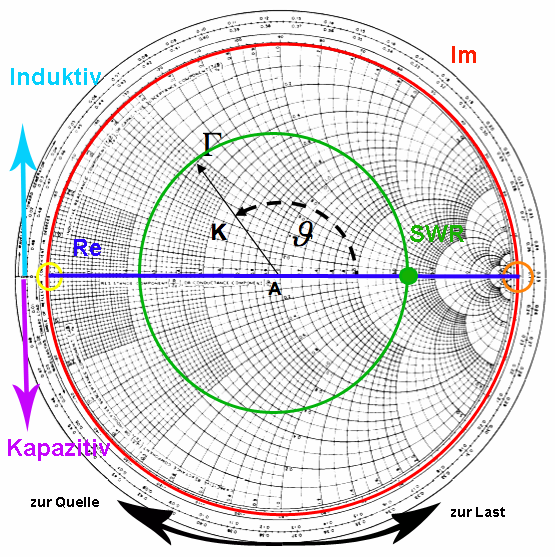
\includegraphics[height=7cm]{./bilder/SmithChart2.png}\\ \\
        	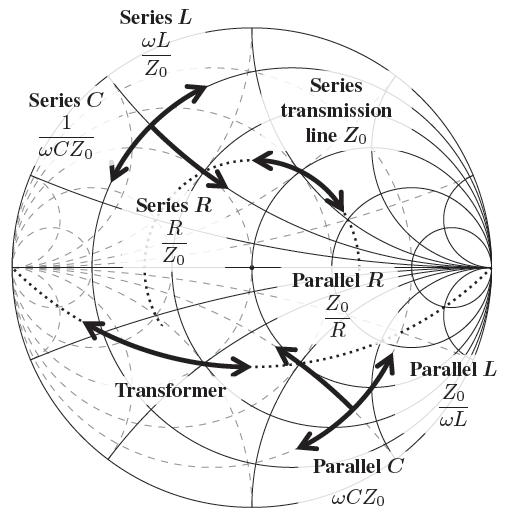
\includegraphics[height=7cm]{./bilder/smith_anpassung.png}
        \end{minipage}
	\end{tabular}
	
	
	\subsection{Anpassungen mit Smith-Chart}
	\begin{multicols}{2}
		\subsubsection{Anpassung durch Längs- und Querreaktanz}
			\parbox[c]{5cm}{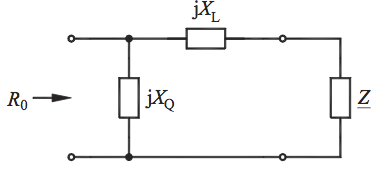
\includegraphics[width = 5cm]{./bilder/Anp_Laengs_Querreaktanz}} \parbox[c]{4cm}{Mit Längsreaktanz auf gespiegelten Kreis (Impedanzebene)}\\
			Auf Fehlabschlüsse mit $Re(\underline{Z}_N)<1$ beschränkt.
		\subsubsection{Anpassung durch Quer- und Längsreaktanz}
			\parbox[c]{5cm}{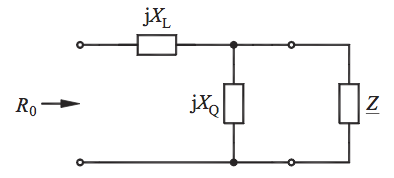
\includegraphics[width = 5cm]{./bilder/Anp_Quer_Laengsreaktanz}}
			\parbox[c]{4cm}{Mit Querreaktanz auf gespiegelten Kreis (Admittanzebene)}\\
			Auf Fehlabschlüsse mit $Re(\underline{Z}_N)>1$ beschränkt.
			\columnbreak
		\subsubsection{Anpassung durch Leitungsstück und Längsreaktanz}
			\parbox[c]{4.5cm}{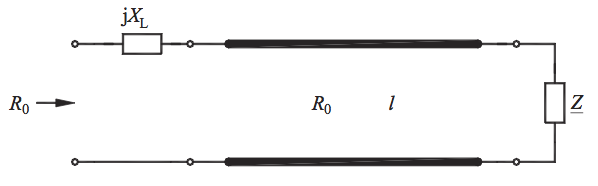
\includegraphics[width = 4.5cm]{./bilder/Anp_Leitung_Laengsreaktanz}
			Durch Leitungsstück auf $Re(\underline{Z}_N)=1$-Kreis transformieren (Impedanzebene)} \hspace{0.5cm}
			\parbox[c]{4.5cm}{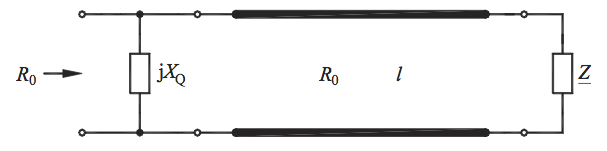
\includegraphics[width = 4.5cm]{./bilder/Anp_Leitung_Querreaktanz}
			Durch Leitungsstück auf $Re(\underline{Y}_N)=1$-Kreis transformieren (Admittanzebene)}
		\subsection{Anpassung durch $\lambda/4$-Transformation}
			\parbox[c]{5cm}{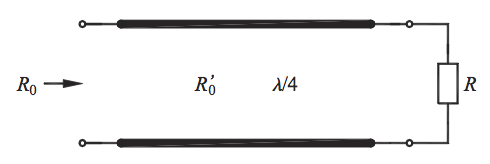
\includegraphics[width = 5cm]{./bilder/Anp_lambda_4_Transfor}}
			\parbox[c]{4cm}{$\frac{R}{R_0'}= \frac{R_0'}{R_0}$\\
			$\Rightarrow R_0' = \sqrt{R \cdot R_0}$}\\
			
	
	\end{multicols}
	
%\subsection{Beispiele bei $Z_0=100\Omega$}
%		\renewcommand{\arraystretch}{1.1}
%		\begin{tabular}{| c | c | c | c | c | c |}
%			\hline
%				\textbf{Fall}
%				& 1
%				& 2 
%				& 3
%				& 4
%				& 5 \\
%			\hline
%				\textbf{LE}
%				& Anpassung
%				& Leerlauf
%				& Kurzschluss
%				& $\lambda/8$ Stichleit. KS
%				& $\lambda/8$ Stichleit. LL \\
%			\hline
%				\textbf{SWR}
%				& 1
%				& $\infty$
%				& $\infty$
%				& $\infty$
%				& $\infty$ \\
%			\hline
%				\textbf{$\underline{r}$}
%				& $0$
%				& $1 \angle 0 ^\circ$
%				& $1 \angle 180 ^\circ$
%				& $1 \angle 90 ^\circ$
%				& $1 \angle 90 ^\circ$\\
%			\hline
%				\textbf{$\underline{Z}_N$}
%				& $1+j0$
%				& $\infty+j\infty$
%				& $0+j0$
%				& $0+j1$
%				& $0-j1$ \\
%			\hline
%				\textbf{$v_{xm}$}
%				& $-$
%				& $\lambda/4$
%				& $\lambda/2$
%				& $3\lambda/8$
%				& $\lambda/8$ \\
%			\hline
%				\textbf{Grafik}
%				& 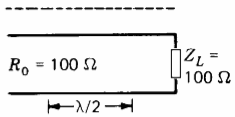
\includegraphics[height=0.9cm]{./bilder/Fall1.png}
%				& 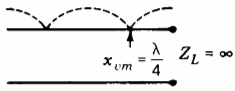
\includegraphics[height=0.9cm]{./bilder/Fall2.png}
%				& 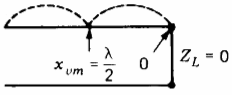
\includegraphics[height=0.9cm]{./bilder/Fall3.png}
%				& 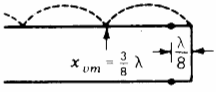
\includegraphics[height=0.9cm]{./bilder/Fall4.png}
%				& 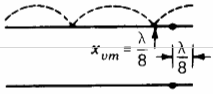
\includegraphics[height=0.9cm]{./bilder/Fall5.png} \\
%			\hline
%		\end{tabular}
%		\renewcommand{\arraystretch}{1}
		